\documentclass{beamer}

\mode<presentation> 
{
    \usetheme{Madrid}
}

\usepackage[utf8x]{inputenc}
\usepackage[english,russian]{babel}
\usepackage[T2A]{fontenc}
\usepackage{graphicx}
\usepackage{booktabs} 
\usepackage{mathtools}
\usepackage{amsmath}
\usepackage{wasysym}
\usepackage{subfig}
\usepackage{hyperref}
\usepackage{ulem}
\usepackage{ragged2e}
\usepackage{algorithm2e}
\usepackage{minted}


\DeclarePairedDelimiter\ceil{\lceil}{\rceil}
\DeclarePairedDelimiter\floor{\lfloor}{\rfloor}


\usemintedstyle{borland}

\usefonttheme[onlymath]{serif}

\hypersetup
{
    colorlinks=true,
    linkcolor=white, 
    urlcolor=cyan
}

\title[Лекция 6]
{
    Лекция 6: Рекусивные структуры данных и динамическая память в языке Си
} 


\author[Д. А. Караваев]{Д. А. Караваев}

\institute[СПбГУТ] 
{
    Санкт-Петербургский государственный университет телекоммуникаций \\ им. проф. М. А. Бонч-Бруевича \\ 
    \vspace{0.2cm}
    Факультет РТС, Кафедра РОС \\
    \vspace{0.2cm}
    Факультатив <<Программирование в ЦОС>> \\
    \vspace{0.2cm}
    Осень 2019
}

\date[25.11.2019]{25.11.2019 Санкт-Петербург} 

\begin{document}
    \begin{frame}
        \titlepage 
    \end{frame}
    \begin{frame}[fragile]
        \frametitle{Cвязные списки}
        \justifying
        Простейшим примером {\it рекурсивной} структуры данных является {\bf однонаправленный связный список}, который состоит из {\it головы} и {\it хвоста}, который также является связным списком, либо отсутствует.
        \begin{figure}[!tbp]
           \centering
           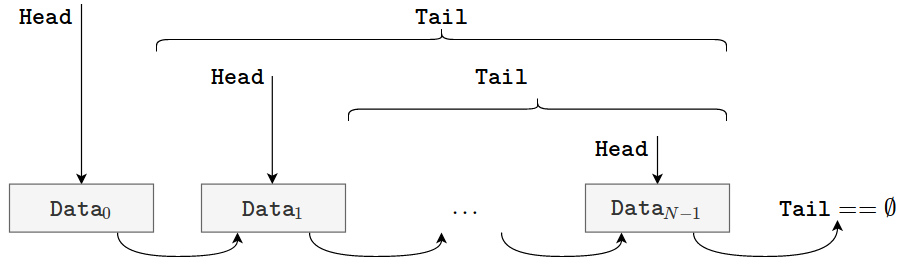
\includegraphics[width=\textwidth]{pics/forward_list.png}
        \end{figure}
    \end{frame}
    \begin{frame}[fragile]
        \frametitle{Реализация в язык Си}
        \justifying
        Односвязный список можно реализовать через структуру, в которой содержится {\it указатель} на хвост.
        \begin{minted}[frame=lines,         framesep=2mm,
                       baselinestretch=1.2, fontsize=\footnotesize,
                       linenos]{c}
/* Определение списка: */
typedef struct list_impl 
{
    int data; /* Содержимое головы. */
    struct list_impl* tail; /* Хвост. */
} list_impl_t;
/* Создание головы: */
list_impl_t head = {.data = 100, .tail = NULL}; /* Нулевой указатель! */
/* Создание хвоста: */
list_impl_t tail = {.data = 200, .tail = NULL};
/* Добавление хвоста: */
head.tail = &tail; 
        \end{minted}
    \end{frame}
    \begin{frame}[fragile]
        \frametitle{Инкапсуляция работы со списком}
        \justifying
        \begin{minted}[frame=lines,         framesep=2mm,
                       baselinestretch=1.2, fontsize=\footnotesize,
                       linenos]{c}
/* Управляющая структура с головой списка (данные): */
typedef struct 
{
    list_impl_t* head; /* Голова списка. */
    size_t       size; /* Число элементов в списке. */
} list_t;
/* Методы: */
/* Добавить элемент в конец списка: */
void list_emplace_back(list_t* list, int data);
/* Подсчитать число элементов в списке с данным значением: */
size_t list_count(const list_t* list, int data);
/* Узнать значение по номеру: */
int list_at(const list_t* list, size_t index);
/* Удалить элемент из списка по номеру: */
void list_delete(list_t* list, size_t index);
        \end{minted}
    \end{frame}
    \begin{frame}[fragile]
        \frametitle{Двунаправленный связный список}
        \justifying
        \begin{minted}[frame=lines,         framesep=2mm,
                       baselinestretch=1.2, fontsize=\footnotesize,
                       linenos]{c}
typedef struct list_impl 
{
    int data; /* Содержимое головы. */
    struct list_impl* succ; /* Последующий элемент. */
    struct list_impl* pred; /* Предыдущий элемент. */
} list_impl_t;
/* Создание списка: */
list_impl_t first = {.data = 100, .succ = NULL, .pred = NULL};
list_impl_t second = {.data = 200, .succ = NULL, .pred = &first};
first.succ = &second;
        \end{minted}
        \begin{figure}[!tbp]
           \centering
           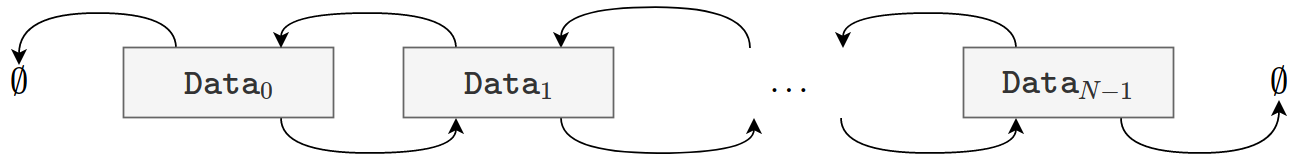
\includegraphics[width=\textwidth]{pics/list.png}
        \end{figure}
    \end{frame}
    \begin{frame}[fragile]
        \frametitle{Замечания по поводу работы со списками}
        \begin{enumerate}
            \justifying
            \item {\bf Алгоритмическая сложность}: Большинство операций в списках имеют $O(N)$ или $\Theta(N)$ временную сложность;
            \item {\bf Реализация стека и очереди}: Списки удобно использовать для реализации стека (или очереди), так как число элементов неограничено;
            \item {\bf Операции c двунаправленным списком}: Можно определить большое множество полезных операций с двунаправленным списком, которые можно реализовать быстрее (с точки зрения алгоритмической сложности) чем для однонаправленного списка;
            \item {\bf Хранение "тяжелых"\ структур}: Списки удобны для хранения структур (пользовательских типов) с большим количеством полей, к которым нет необходимости применять индексацию.
        \end{enumerate}
    \end{frame}
    \begin{frame}[fragile]
        \frametitle{Дерево бинарного поиска}
        \justifying
        Другим примером рекурсивной структуры данных служит {\bf дерево}, которое состоит из {\bf корня} (родителя), в котором хранится значение ({\it ключ}) и у которого может быть несколько {\bf поддеревьев} (потомков). Деревья, у которых нет поддеревьев, называются {\bf листьям}.
        \par
        \vspace{0.5cm}
        \par
        \justifying
        Если у дерева может быть не более двух поддеревьев, и {\it для каждого родительского ключа ключи большее него храняться в правом поддереве, а меньше в левом}, то таком дерево называется {\bf деревом бинарного поиска}. Все значения в дереве {\it уникальны}.
    \end{frame}
    \begin{frame}[fragile]
        \frametitle{Иллюстрация дерева бинарного поиска}
        \begin{figure}[!tbp]
           \centering
           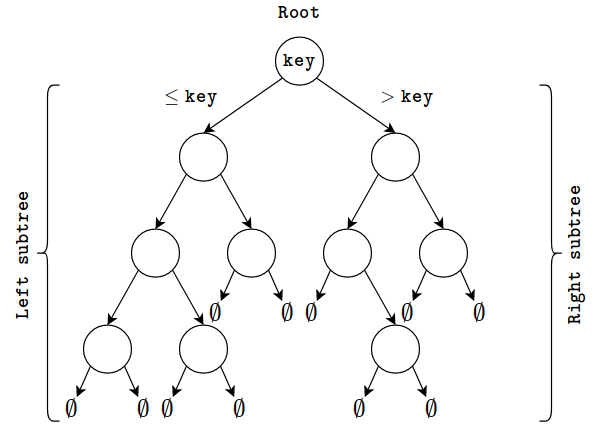
\includegraphics[width=0.85\textwidth]{pics/tree.png}
        \end{figure}
    \end{frame}
    \begin{frame}[fragile]
        \frametitle{Представление дерева бинарного поиска в языке Си}
        \begin{minted}[frame=lines,         framesep=2mm,
                       baselinestretch=1.2, fontsize=\footnotesize,
                       linenos]{c}
typedef struct bstree_node
{
    int key; /* Ключ. */
    struct bstree_node* left; /* Левое поддерево. */
    struct bstree_node* rigth; /* Правое поддерево. */
} bstree_node_t;
/* Управляющая структура с корнем дерева: */
typedef 
{
    bstree_node_t* root; /* Корень дерева. */
    size_t size; /* Размер дерева. */
} bstree_t;
void bstree_emplace(bstree_t* tree, int key); /* Добавить элемент. */
int bstree_find(const bstree_t* tree, int key); /* Найти элемент. */
void bstree_delete(bstree_t* tree, int key); /* Удалить элемент. */
        \end{minted}
    \end{frame}
    \begin{frame}[fragile]
        \frametitle{Замечания к дереву бинарного поиска}
        \begin{enumerate}
            \justifying
            \item {\bf Алгоритмическая сложность}:
            Если дерево заполнено равномерно, то алгоритмическая сложность всех операций пропорциональна его выcоте $O(h) = O(\log N)$, где $N$ - число элементов в дереве.
            \item {\bf Разбалансировка}:
            Явление, при котором основная "масса"\ элементов дерева сосредоточена вдоль одного края (ветви). Таким образом, дерево {\it вырождается} в однонаправленный список и преимущество в скорости поиска элементов теряется. Для борьбы с этим явлением используют более сложные реализации бинарных деревьев (красно-черные и AVL деревья).
            \item {\bf Ассоциативный контейнер}:
            Деревья часто используются для реализации {\it ассоциативного контейнера (словарь)}, в котором тип индекса ({\it ключа}) может быть любым упорядоченным типом (например, строкой).
        \end{enumerate}
    \end{frame}
    \begin{frame}[fragile]
        \frametitle{Иллюстрация разбалансировки}
        \begin{figure}[!tbp]
           \centering
           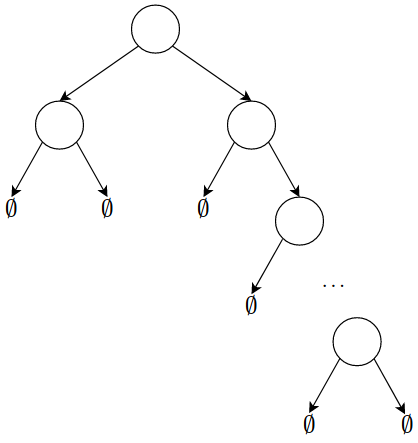
\includegraphics[width=0.6\textwidth]{pics/inbalance.png}
        \end{figure}
    \end{frame}
    \begin{frame}[fragile]
        \frametitle{Реализации вставки в односвязный список}
        \begin{minted}[frame=lines,         framesep=2mm,
                       baselinestretch=1.2, fontsize=\footnotesize,
                       linenos]{c}
void list_emplace_back(list_t* list, int data)
{
    list_emplace_back_impl(list->head, data);
    list->size += 1;
}
void list_emplace_back_impl(list_impl_t* head, int data)
{
    if (head->tail == NULL)
    {
        list_impl_t tail = {.data = data, .tail = NULL};
        head->tail = &tail; /* Ошибка. tail - локальная переменная! */
        return;
    }
    list_emplace_back_impl(head->tail, data);
}
        \end{minted}
    \end{frame}
    \begin{frame}[fragile]
        \frametitle{Динамическая память}
        \justifying
        {\bf Определение}: Память, выделяемая операционной системой (ОС) для {\bf всего} приложения, в которой можно размещать данные заданного размера ({\it возможно неизвестного на этапе написания программы!}).
        \begin{minted}[frame=lines,         framesep=2mm,
                       baselinestretch=1.2, fontsize=\footnotesize,
                       linenos]{c}
/* Считываем размер данных с терминала: */
size_t N;
scanf("%lu", &N);
/* Для выделения участка память в динамической памяти (куче от англ. heap)
 * используется функция malloc: */
/* Получаем указатель на первый элемент! */
int* array = (int*)malloc(sizeof(int) * N); 
/* Инициализация и обработка ... */
/* После работы выделенный блок памяти должен быть освобожден! */
free(array);
/* При помощи malloc можно создать экземпляр любого типа в куче. */
        \end{minted}
    \end{frame}
    \begin{frame}[fragile]
        \frametitle{Замечания по поводу динамической памяти}
        \begin{enumerate}
            \justifying
            \item {\bf Динимические массивы}: возможность создания массивов различной длины, которая может меняться по ходу исполнения программы;
            \item {\bf Скорость работы}: выделение дианамической памяти требует значительного времени по сравнению с созданием переменных в (программном) стеке и зависит от ОС;
            \item {\bf Утечки памяти}: проблема, при которой уже неиспользуемая память не была освобождена, что может приводить к {\bf очень серьёзным} проблемам;
            \item {\bf Фрагментация памяти}: при частом размещении/удалении переменных в куче возникает проблема фрагментации памяти;
            \item {\bf Иерархия памяти}: на некоторых вычислительных устройствах существуют различные типы куч (по скорости доступа и объёму).
        \end{enumerate}
    \end{frame}
    \begin{frame}[fragile]
        \frametitle{Реализации вставки в односвязный список (+ динамическая память)}
        \begin{minted}[frame=lines,         framesep=2mm,
                       baselinestretch=1.2, fontsize=\footnotesize,
                       linenos]{c}
void list_emplace_back_impl(list_impl_t* head, int data)
{
    if (head->tail == NULL)
    {
        list_impl_t* tail = (list_impl_t*)malloc(sizeof(list_impl_t));
        tail->data = data;
        tail->tail = NULL:
        head->tail = tail;
        return;
    }
    list_emplace_back_impl(head->tail, data);
}
/* NB: В момент удаления элемента должна быть вызвана free! */
        \end{minted}
    \end{frame}
    \begin{frame}[fragile]
        \frametitle{Задание}
        {\bf Реализовать}:
        \begin{enumerate}
            \justifying
            \item Функции (методы) вставки, удаления, поиска для односвязного списка;
            \item Функции (методы) вставки, удаления, поиска для дерева бинарного поиска;
        \end{enumerate}
        \par
        {\bf Домашнее задание}: 
        \begin{enumerate}
            \justifying
            \item Реализовать аналогичные методы для двунаправленного списка;
            \item Реализовать стек и/или очередь с использованием связного списка;
            \item {\bf*} Реализовать красно-черное дерево и функции к нему.
        \end{enumerate}
        \par
        {\bf Проект}: Решение задачи необходмо поместить в файл {\tt source/main.c} в проекте {\tt Tree}. 
    \end{frame}
    \begin{frame}
        \begin{center}
        \baselineskip 20.0mm
        \Huge Спасибо за внимание!
        \end{center}
    \end{frame}
\end{document}
